\section{Additional Diagnostic Figures}
\label{app:diagnostic-figures}

\subsection{Branched High-\texorpdfstring{$k$}{k} Helmholtz Diagnostic}

The branched Helmholtz campaign records the local branch probe used in the
main text.  It tests whether the high-$k$ Helmholtz stress row is improved by
a finite outgoing-branch implementation at the sample-capped budget used in
the manuscript.

\begin{table}[t]
\centering
\caption{Branched MiNO high-$k$ Helmholtz diagnostic. Entries are mean relative $\ell^2$ over available seeds under the local sample-capped protocol; lower is better. The table tests whether finite canonical-branch structure reduces the high-$k$ gap at this budget, not a global Helmholtz resolvent theorem or full-budget benchmark.}
\label{tab:helmholtz-branched-highk}
\scriptsize
\begin{tabular}{lcccccc}
\toprule
Scenario & Full & Single br. & Uniform route & No tr. & No tr./car. & No sym. \\
\midrule
Helm. high-k ctl. & 0.548 & 0.548 & 0.548 & 0.559 & 0.554 & 0.548 \\
Helm. high-k & 0.705 & 0.705 & 0.705 & 0.706 & 0.722 & 0.705 \\
Helm. var.+ & 0.735 & 0.735 & 0.735 & 0.735 & 0.734 & 0.735 \\
\bottomrule
\end{tabular}
\end{table}


\begin{figure}[t]
\centering
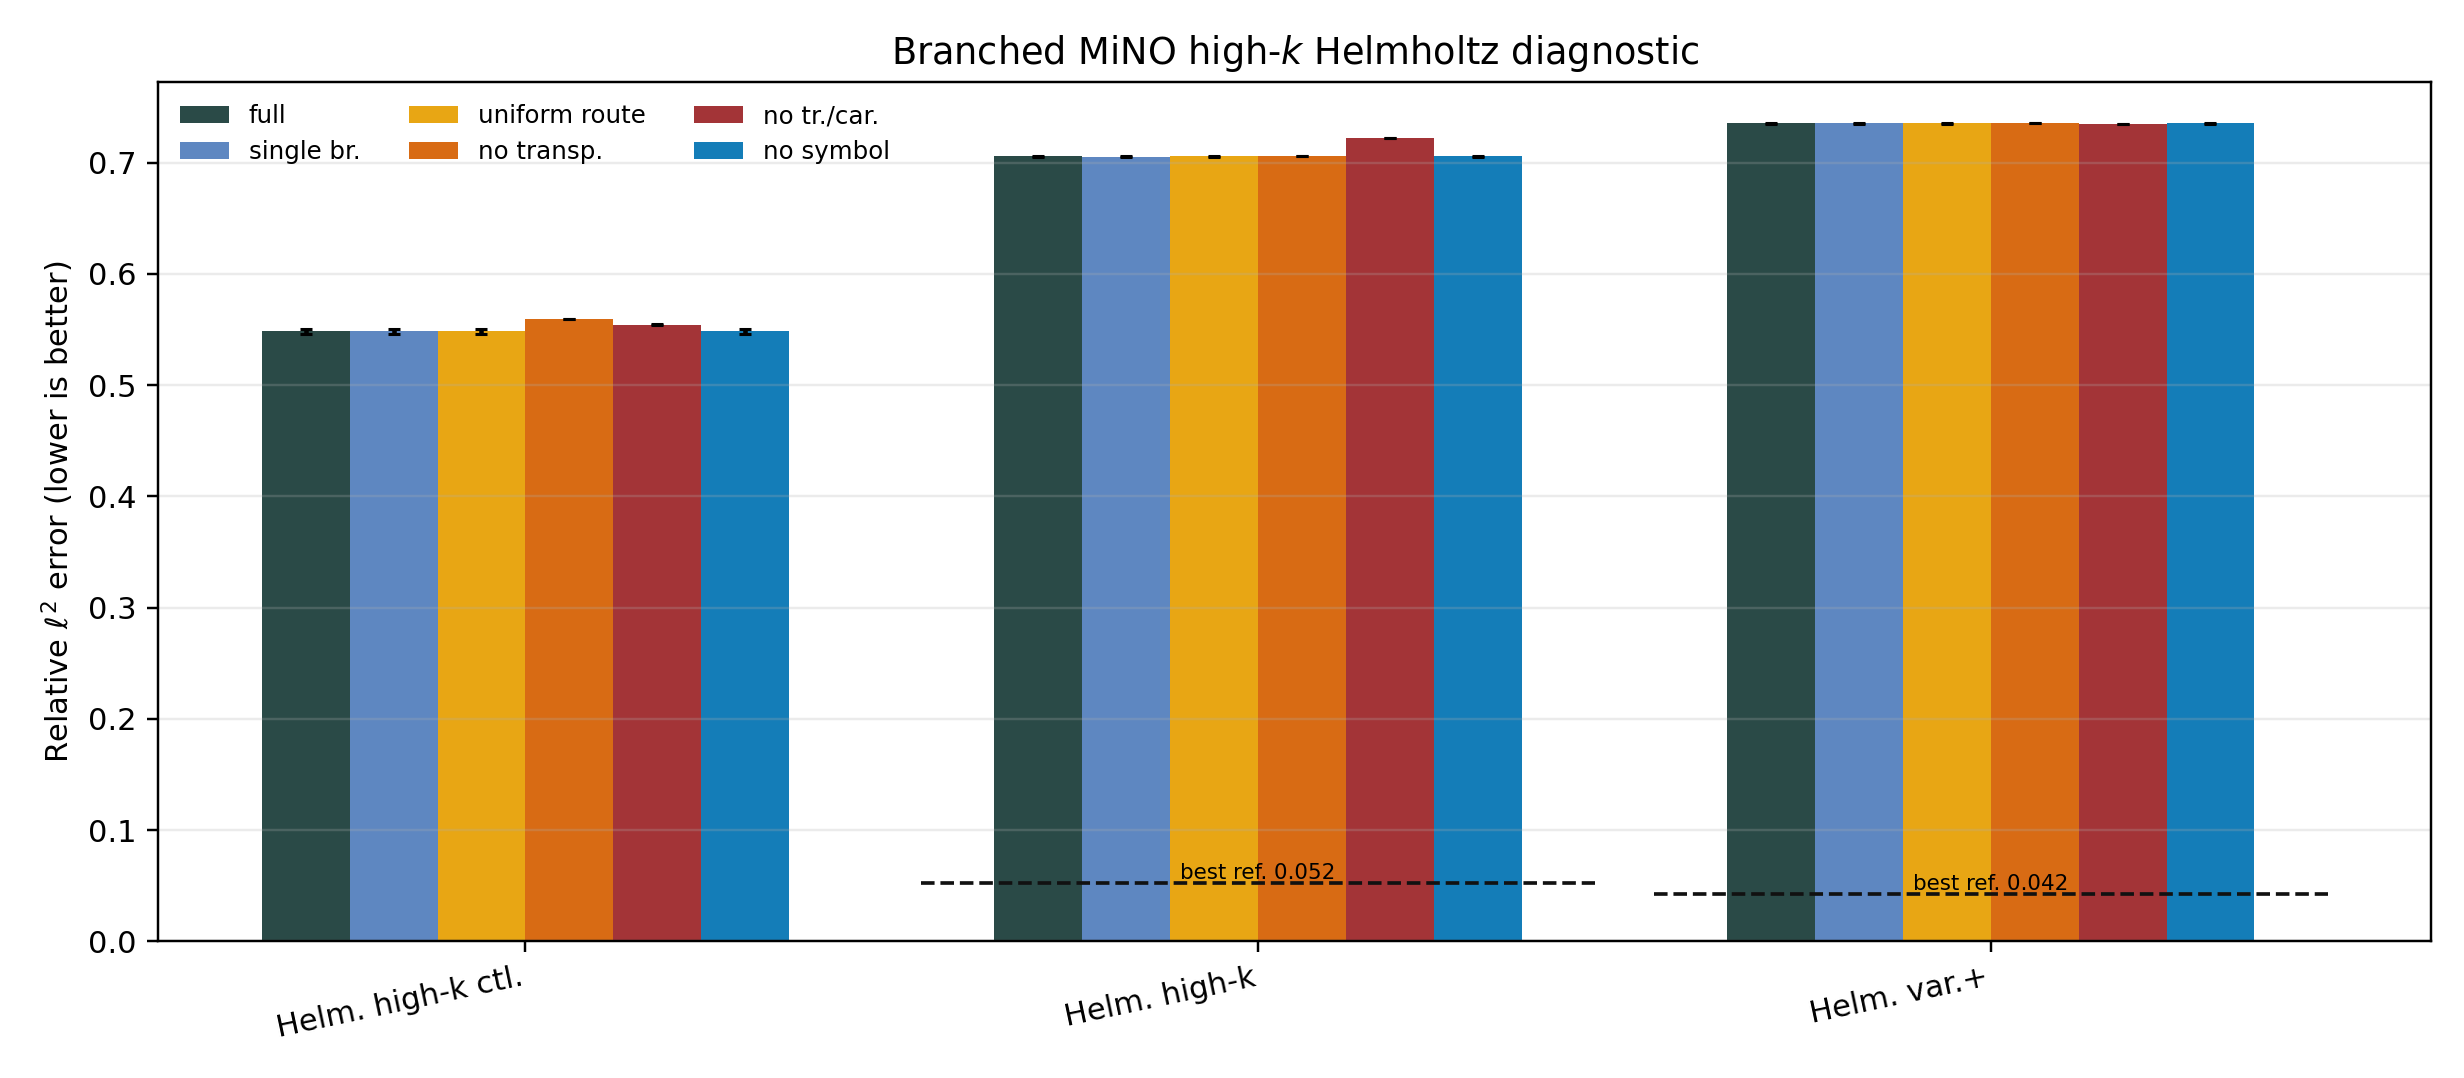
\includegraphics[width=\textwidth]{figures/helmholtz_branched_highk_relative_l2.png}
\caption{Branched \MiNO\ high-$k$ Helmholtz diagnostic.  The figure compares the full branched carrier-bound model against single-branch, uniform-routing, transport-removal, carrier-removal, and symbol-removal ablations under the local sample-capped protocol.  Dashed reference marks are imported baselines where available.}
\label{fig:helmholtz-branched-highk}
\end{figure}

\begin{figure}[t]
\centering
\begin{minipage}{0.49\linewidth}
\centering
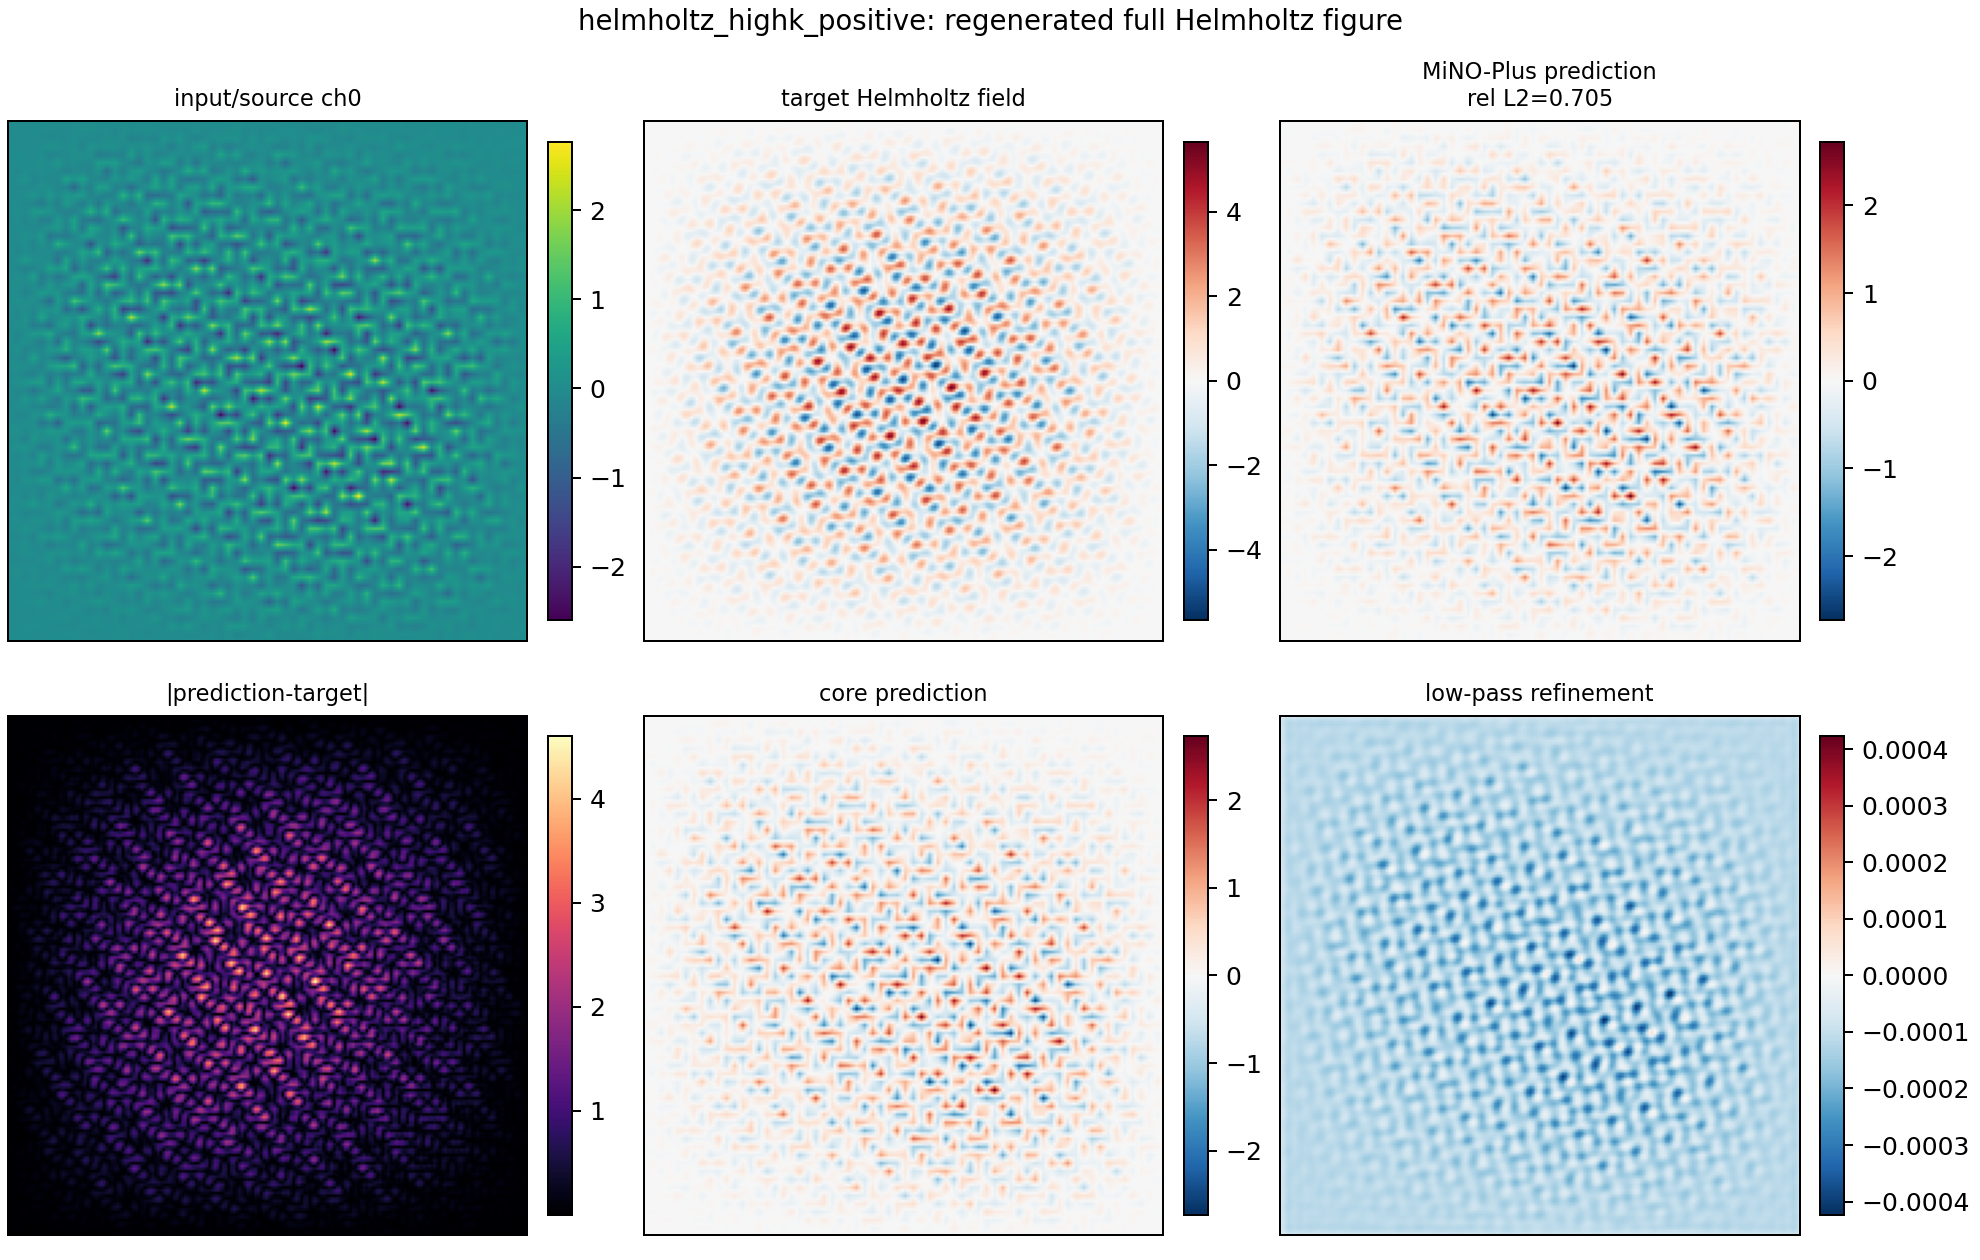
\includegraphics[width=\linewidth]{figures/helmholtz_highk_positive_seed7_sample0_anisotropic_gabor_full_L3.png}
\end{minipage}
\hfill
\begin{minipage}{0.49\linewidth}
\centering
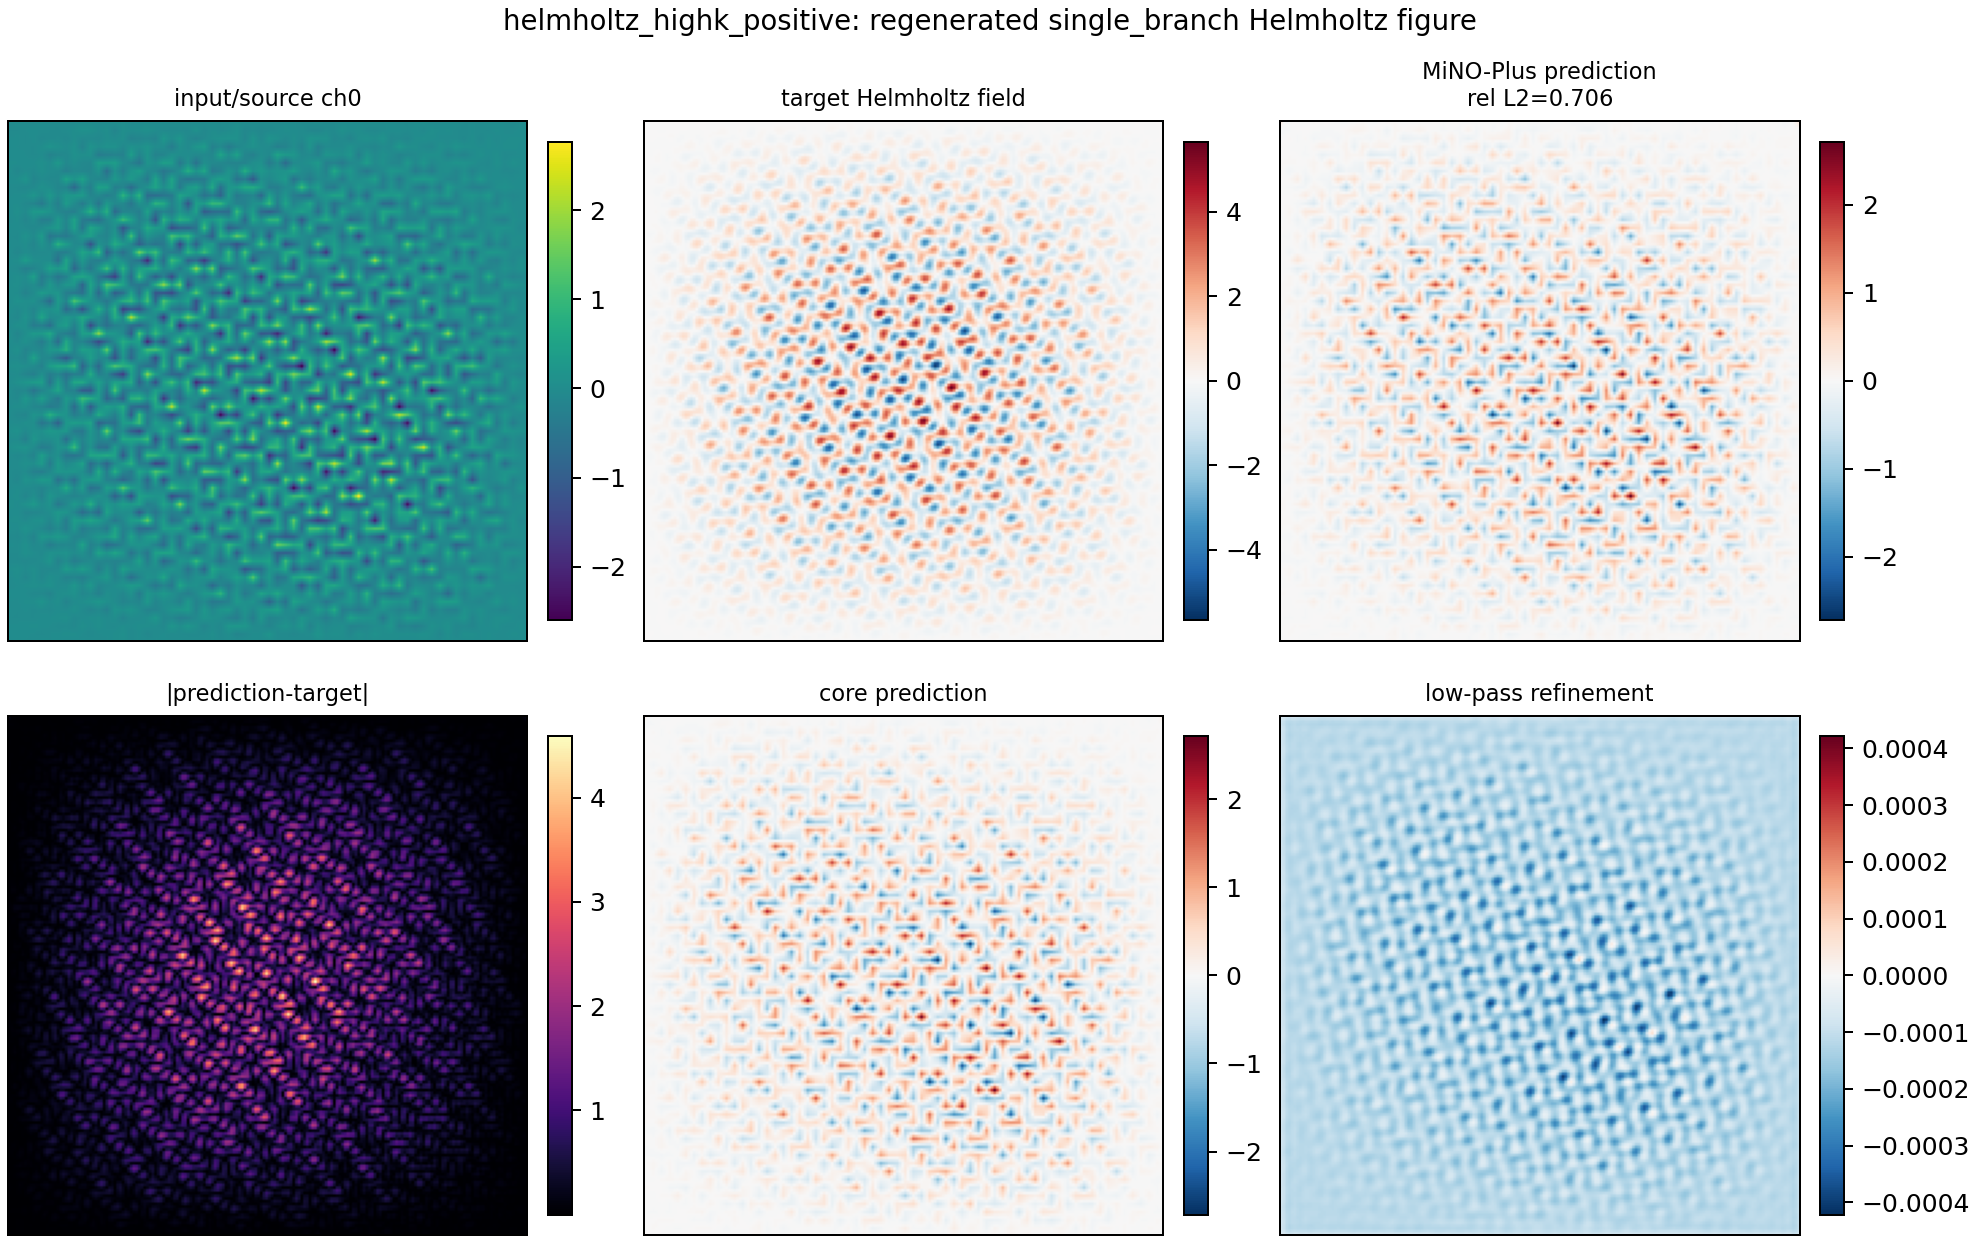
\includegraphics[width=\linewidth]{figures/helmholtz_highk_positive_seed7_sample0_anisotropic_gabor_single_branch_L3.png}
\end{minipage}
\caption{High-$k$ Helmholtz prediction panels for the sample-capped branched diagnostic.  Left: full $L=3$ branched model.  Right: forced single-branch control at the same budget and sample.  The nearly identical relative errors show that branch multiplicity alone leaves the main high-$k$ correction budget to the frame, router, phase/landing, and resolvent-symbol terms.}
\label{fig:helmholtz-branched-predictions}
\end{figure}

\subsection{Low-Budget Calculus-Regime Diagnostics}

The following panels are stress diagnostics for local-window Helmholtz and
synthetic Navier--Stokes profiles.  They are included to document boundary
conditions for future calculus hooks, not as main success claims.

\begin{figure}[t]
\centering
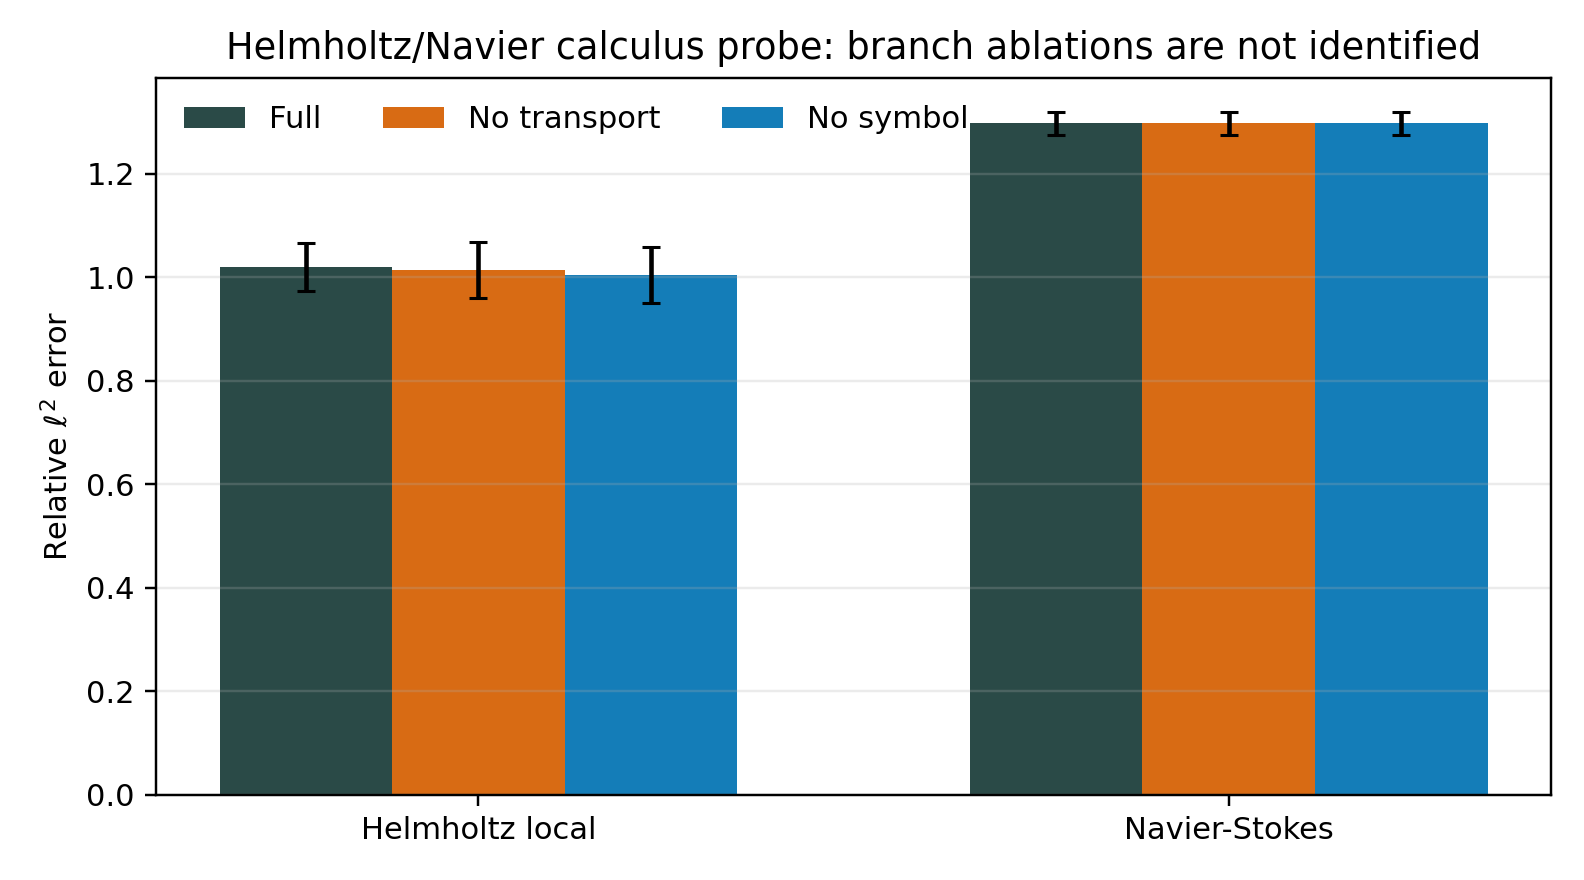
\includegraphics[width=0.82\textwidth]{figures/helmholtz_navier_calculus_probe.png}
\caption{Low-budget calculus-regime probe on local-window Helmholtz and synthetic Navier--Stokes.  Each row uses three seeds, twelve epochs, and restricted train/validation/test samples.  The nearly flat ablation bars identify which branch effects are not active at this scale and motivate the dedicated branch/resolvent and transport--diffusion profiles.}
\label{fig:helmholtz-navier-calculus-probe}
\end{figure}

\begin{figure}[t]
\centering
\begin{minipage}{0.49\linewidth}
\centering
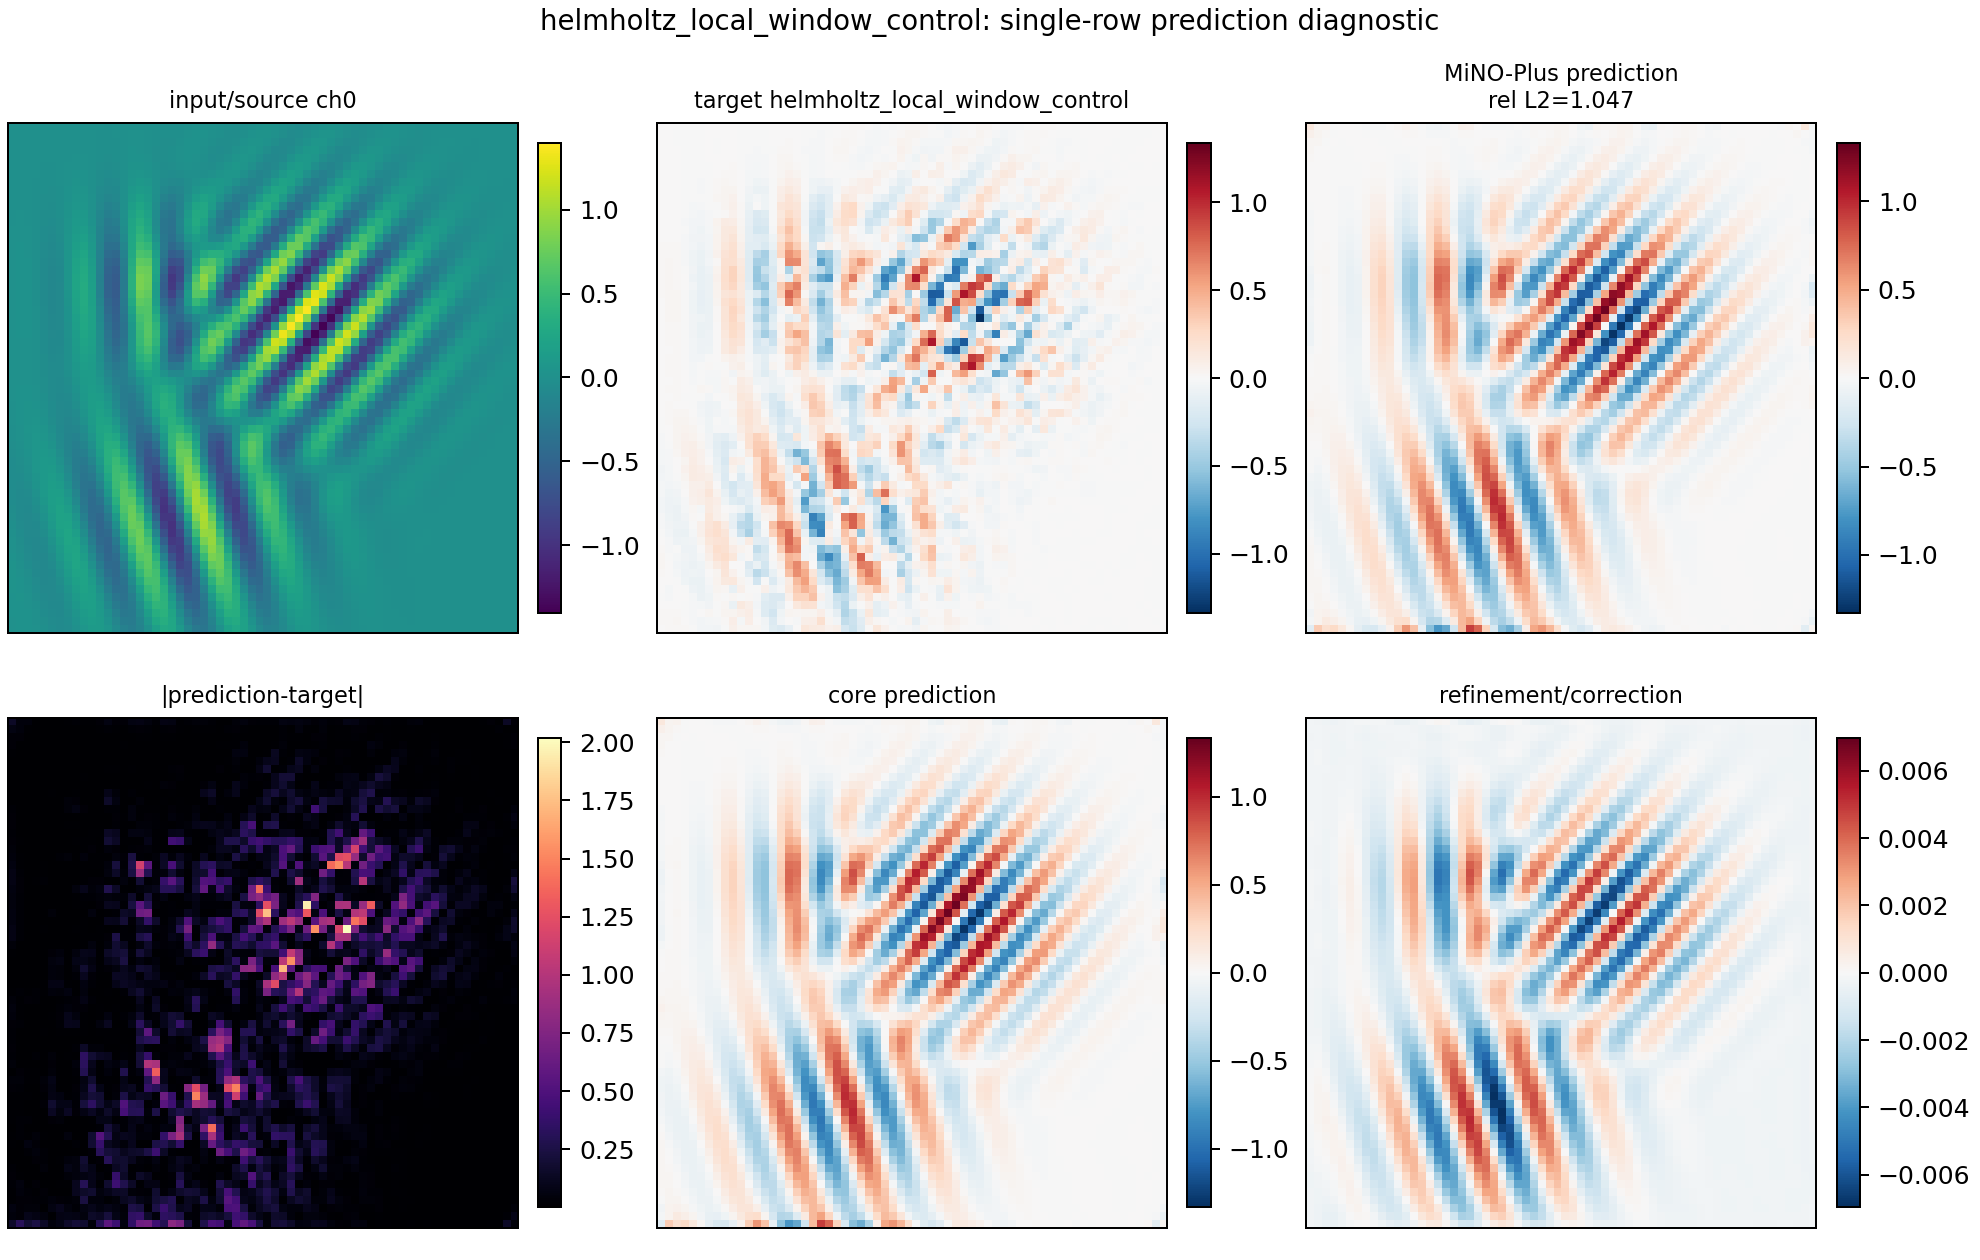
\includegraphics[width=\linewidth]{figures/helmholtz_local_window_prediction.png}
\end{minipage}
\hfill
\begin{minipage}{0.49\linewidth}
\centering
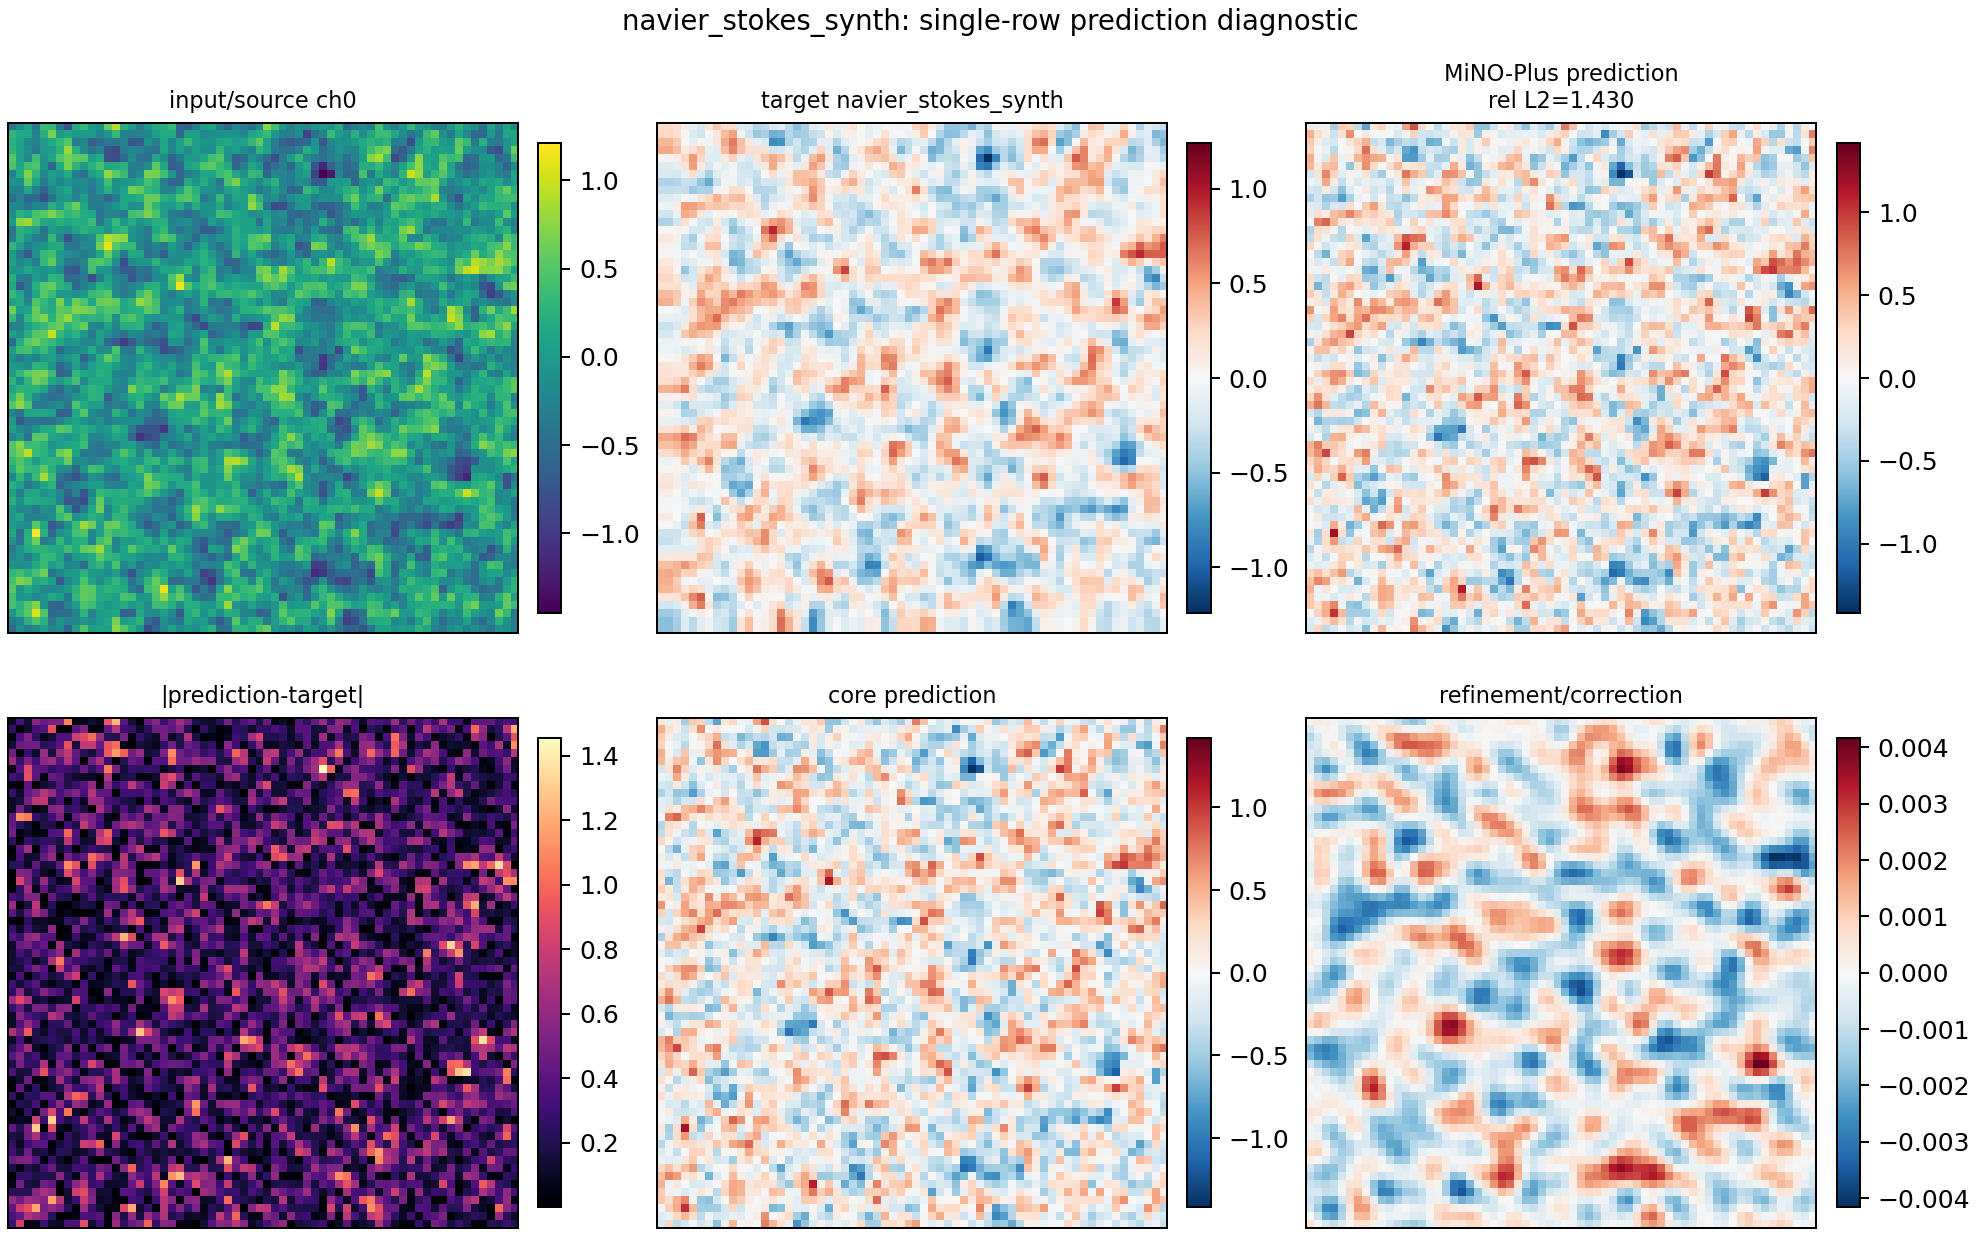
\includegraphics[width=\linewidth]{figures/navier_stokes_prediction.png}
\end{minipage}
\caption{Single-row prediction diagnostics for the same low-budget Helmholtz/Navier probe.  The panels visualize input, target, prediction, absolute error, core prediction, and refinement/correction for one held-out sample.  These rows show the regimes that motivate the next calculus hooks.}
\label{fig:helmholtz-navier-prediction-panels}
\end{figure}

\clearpage
